\chapter{mcmcreg objects}
\label{mcmcreg} \index{mcmcreg object}



{\em mcmcreg objects} are used to fit (multivariate) distributional regression models with {\em
structured additive predictor}, see \citeasnoun{kleknelan14a}. Hierarchical data structures may be considered using
hierarchical or multilevel structured additive predictors. For multilevel structured additive models  see
\citeasnoun{LanUml14}. Inference is based on a fully Bayesian approach implemented via Markov Chain Monte Carlo (MCMC)
simulation techniques. The methodology manual provides a brief introduction to structured additive regression and MCMC-based
inference. More details can be found in the references cited above and in the book by \citeasnoun{fahkne13}

First steps with {\em mcmcreg objects} can be done with the
tutorial like example in chapter ?? of the
tutorials manual which provides a self-contained demonstrating
example.


\clearpage

\section{Method hregress}
\label{mcmcregress} \index{mcmcreg object!hregress
function}\index{hregress function}

\subsection{Description}
\label{mcmcregregressdescr}

Method #hregress# estimates distributional structured additive regression models.

\index{Generalized linear models} \index{Generalized additive
models} \index{Varying coefficients} \index{Bayesian semiparametric
regression} \index{MCMC} \index{Markov chain Monte Carlo}
\index{Distributional regression}

\subsection{Syntax}
\index{Regression syntax}\index{mcmcreg object!Regression syntax}
\label{mcmcregregresssyntax}

 #> #{\em objectname}.#hregress# {\em model} [#weight# {\em weightvar}] [#if# {\em expression}] [{\em , options}] #using# {\em dataset}

Method #hregress# estimates the regression model specified in {\em
model} using the data specified in {\em dataset}. {\em dataset}
has to be the name of a {\em dataset object} created before. The
details of correct models are covered in \autoref{mcmcregmodelsyntax}.
The distribution of the response variable can be chosen from a wide
range of uni- and multivariate distributions. It is
specified using option
#family#, see \autoref{mcmcregfamilysyntax} below and the options list in
\autoref{mcmcregregressoptions}. The default value is #family=gaussian#
with an identity link. An #if# statement may be specified to analyze
only parts of the data set, i.e.~the observations where {\em
expression} is true.

\subsubsection{Optional weight variable}\index{Weighted regression}
\label{weightspecification}

An optional weight variable {\em weightvar} may be specified to
estimate weighted regression models.


%For Gaussian responses {\em
%BayesX} assumes that $y_r|\eta_r,\sigma^2 \sim
%N(\eta,\sigma^2/weightvar_r)$. Thus, for grouped Gaussian
%responses the weights must be the number of observations in the
%groups if the $y_r$'s are the average of individual responses. If
%the $y_r$'s are the sum of responses in every group, the weights
%have to be the reciprocal of the number of observations in the
%groups. Of course, estimation of usual weighted regression models
%with heteroscedastic errors is also possible. In this case the
%weights should be proportional to the reciprocal of the
%heteroscedastic variances. If the response distribution is
%binomial, it is assumed that the values of the weight variable
%correspond to the number of replications and that the values of
%the response variable itself correspond to the number of
%successes. If #weight# is omitted, {\em BayesX} assumes that the
%number of replications is one, i.e.~the values of the response
%must be either zero or one. For grouped Poisson data the weights
%have to be the number of observations in a group and the $y_i$'s
%are assumed to be the average of individual responses. In the case
%of gamma distributed responses, {\em BayesX} assumes $y_r \sim
%G(\exp(\eta_r),\nu/weightvar_r)$ where $\mu_r= \exp(\eta_r)$ is
%the mean and $s_r = \nu/weightvar_r$ is the scale parameter.
%
%If estimation is based on latent utility representations, the
%specification of weights is not allowed. Similarly, for negative
%binomial, zero inflated Poisson and zero inflated negative
%binomial models as well as hazard regression and multi-state
%models, weighted regression is not implemented yet.

\subsubsection{Syntax of possible model terms}
\label{mcmcregmodelsyntax}\index{Model terms}\index{mcmcreg object!Model
terms}

The general syntax of models is:

$depvar = term_1 + term_2 + \cdots + term_r$

where {\em depvar} specifies the dependent variable in the model
and $term_1$,\dots,$term_r$ define the specific form of covariate
effects on the dependent variable. The different terms have to be
separated by '+' signs. A constant intercept is (in contrast to
{\em bayesreg objects}) NOT automatically
included in the models and must be specified by the
user. This section reviews all possible model terms that are
currently supported by {\em mcmcreg objects} and provides some
specific examples. Note that all described terms may be combined
in arbitrary order. An overview about the capabilities of {\em
mcmcreg objects} is given in \autoref{mcmcterms}.

\autoref{mcmcreginteractions} shows how interactions between
covariates are specified. Full details about all available options
are given in \autoref{mcmclocaloptions}.

Throughout this section #Y# will denote the dependent variable.

\subsubsection*{Offset}\index{Offset}

\begin{itemize}
\item[] {\em Description}: Adds an offset term to the predictor.
\item[] {\em Predictor}: $\eta =  \cdots + \mbox{\it offs} + \cdots$
\item[] {\em Syntax}: #offs(offset)#
\item[] {\em Example}:

The following model statement can be used to estimate a Poisson
model with #offs# as offset term and #W1# and #W2# as fixed
effects (if #family=poisson# is specified in addition):

#Y = offs(offset) + W1 + W2#

\end{itemize}

\subsubsection*{Fixed effects}\index{Fixed effects}

\begin{itemize}
\item[] {\em Description}: Incorporates covariate #W1# as a fixed effect into the model.
\item[] {\em Predictor}: $\eta =  \cdots + \gamma_1 W1 + \cdots$
\item[] {\em Syntax}: #W1#
\item[] {\em Example}:

The following model statement specified a model with $q$ fixed
(linear) effects:

\texttt{Y = W1 + W2 + $\cdots$ + Wq}
\end{itemize}

% NEW_START: Susanne.Konrath@stat.uni-muenchen.de %%%%%%%%%%%%%%%%%%%%%%%%%%%%%%
STEFAN: NOCHMAL CHECKEN
\subsubsection*{Shrinkage of fixed effects}
\index{Shrinkage of fixed Effects}

\begin{itemize}
\item[] {\em Description}: Defines a shrinkage-prior for the corresponding
  parameters $\gamma _{j} $, $j=1,\ldots,q$, $q \ge 1$ of the linear effects
  #X1,...Xq#. There are three priors possible: ridge-,
  lasso- and Normal Mixture of inverse Gamma (NMIG)-prior.

\item[] {\em Predictor}: $\eta =\cdots +\gamma _{1} {\kern 1pt} X1+\cdots +
  \gamma _{q} {\kern 1pt} Xq+\cdots $

\item[] {\em Syntax}:

  \begin{itemize}
  \item  Ridge-prior: #X1(ridge#[, {\em options}]#) #
  \item  Lasso-prior: #X1(lasso#[, {\em options}]#) #
  \item  NMIG-prior: #X1(nigmix#[, {\em options}]#) #
  \end{itemize}

\item[] {\em Example}:
 The following model statement can be used to estimate a model with $q$ lasso-penalized
 linear effects

 #Y = X1(lasso)+...+ Xq(lasso)#

 By default, the starting value of the shrinkage parameter in the Markov chain is
 set to 1 and the shrinkage parameter is estimated by the data. It is also possible
 to fix the shrinkage parameter through the iterations in order to use a prespecified
 amount for shrinkage. To do so the the option #shrinkagefix# have to be set
 in the corresponding terms and this results in fixing the shrinkage parameter at
 the starting value assigned in the option #shrinkage#.

 The following model term defines a lasso-penalty with shrinkage parameter
 fixed at the value 1.5:

 #Y = X1(lasso)+...+ Xq(lasso,shrinkage=1.5,shrinkagefix)#

 Full details about all possible options for shrinkage-effects are given in \ref{localoptions}.

 {\em Important Remark}: Except the option #tau2# for the variances of lasso or ridge
 (and resp. the options #I# and #t2# for nigmix),
 all the other possible options used in the shrinkage-methods are those which are
 specified in the first term of the corresponding penalty, e.g.

 #Y = X2(lasso,shrinkagepar=2,shrinkagefix)+ X1(lasso,shrinkagepar=1.5)#

 uses the options of #X2#. If the option #adaptive# is specified the options from
 each term are used.

\end{itemize}

% NEW_END: Susanne.Konrath@stat.uni-muenchen.de %%%%%%%%%%%%%%%%%%%%%%%%%%%%%%%%


\subsubsection*{Nonlinear effects of continuous covariates and time scales}
\index{Nonlinear effects}
\index{P-splines}


\begin{itemize}
\item[] {\em Description}: Defines a P-spline with a first or
second order random walk penalty for the parameters of the spline.

\item[] {\em Predictor}: $\eta =  \cdots + f_1(X1) + \cdots$

\item[] {\em Syntax}:
#X1(psplinerw1#[{\em , options}]#) #

#X1(psplinerw2#[{\em , options}]#) #

\item[] {\em Example}:

A P-spline with second order random walk penalty is obtained by:

#Y = X1(pspline)#

By default, the degree of the spline is 3 and the number of inner
knots is 20. The following model term defines a quadratic P-spline
with 30 knots and a first order random walk penalty:

#Y = X1(pspline,degree=2,nrknots=30,difforder=1)#

Full details about all possible options for P-splines are given in
\autoref{mcmclocaloptions}.
\end{itemize}



\subsubsection*{Spatial Covariates}
\index{Spatial effects}
\index{Markov random fields}
%\index{Two-dimensional P-spline}

\begin{itemize}
% \item[]{\bf\sffamily Markov random field}

\item[] {\em Description}:

Defines a Markov random field prior for the spatial covariate
#region#. {\em BayesX} allows to incorporate spatial covariates
with geographical information stored in the {\em map object}
specified in option #map#.

\item[] {\em Predictor}: $\eta = \cdots + f_{spat}(region) +
\cdots$

\item[] {\em Syntax}:

#region(spatial,map=#{\em characterstring}#[#{\em , options}]#) #
\item[] {\em Example}:

For the specification of a Markov random field prior, #map# is an
obligatory argument that represents the name of a {\em map object}
(see \autoref{map}) containing all necessary spatial information
about the geographical map, i.e.~the neighbors of each region and
the weights associated with the neighbors. For example the
statement

#Y = region(spatial,map=germany)#

defines a Markov random field prior for #region# where the
geographical information is stored in the {\em map object}
#germany#. An error will be raised if #germany# is not existing.
It is advisable to reorder the regions of a map prior to
estimation of a spatial effect to obtain a band matrix like
precision matrix. This can be achieved using method #reorder# of
{\em map objects}, see \autoref{mapreorder} for details.



%\item[]{\bf\sffamily Two-dimensional P-spline with first order
%random walk penalty}
%
%\item[] {\em Description}:
%
%Defines a two-dimensional P-spline for the spatial covariate
%#region# with a two-dimensional first order random walk penalty
%for the parameters of the spline. Estimation is based on the
%coordinates of the centroids of the regions. The centroids are
%computed using the geographical information stored in the {\em map
%object} specified in the option #map#.
%
%\item[] {\em Predictor}: $\eta= \cdots + f(centroids) + \cdots$
%
%\item[] {\em Syntax}:
%
%#region(geospline,map=#{\em characterstring}#[, #{\em options}]#) #
%\item[] {\em Example}:
%
%For the specification of a two-dimensional P-spline ({\em
%geospline}) #map# is an obligatory argument indicating the name of
%a {\em map object} (see \autoref{map}) that contains all necessary
%spatial information about the geographical map, i.e.~the neighbors
%of each region and the weights associated with the neighbors. The
%model term
%
%#Y = region(geospline,map=germany)#
%
%specifies a two-dimensional cubic P-spline with first order random
%walk penalty where the geographical information is stored in the
%{\em map object} #germany#.
\end{itemize}


\subsubsection*{Unordered group indicators}
\index{Unordered group indicators}
\index{Random effects}
\index{Random intercept}

STEFAN: MUSS SO NOCH IMPLEMENTIERT WERDEN

\begin{itemize}
\item[]{\bf\sffamily Unit- or cluster-specific unstructured effect}

\item[] {\em Description}: Defines an unstructured (uncorrelated)
random effect with respect to grouping variable #grvar#. \item[]
{\em Predictor}: $\eta = \cdots + f(grvar) + \cdots$ \item[] {\em
Syntax}:

#grvar(random#[, {\em options}]#) #
\item[] {\em Example}:

Gaussian i.i.d.~random effects allow to cope with unobserved
heterogeneity among units or clusters of observations. Suppose the
analyzed data set contains a group indicator #grvar# that gives
information about the individual or cluster a particular
observation belongs to. Then an individual-specific uncorrelated
random effect is defined by

#Y = grvar(random)#

Note that {\em BayesX} allows the specification of hierarchical or multilevel models that go far beyond
the simple random intercept term described above, see section ??.
\end{itemize}



\subsubsection*{Varying coefficients with continuous covariates as
effect modifier}
\index{Varying coefficients}

\begin{itemize}

\item[] {\em Description}:

Defines a varying coefficient term, where the effect of #X1#
varies smoothly over the range of #X2#. The smoothness prior for
$f(X2)$ is a P-spline with first or second order random walk
penalty. \item[] {\em Predictor}: $\eta= \cdots + f(X2)X1 +
\cdots$ \item[] {\em Syntax}:

#X1*X2(pspline#[, {\em options}]#) #

\item[] {\em Example}:

A varying coefficient term with a second order random walk
smoothness prior is defined as follows:

#Y = X1*X2(pspline)#
\end{itemize}


\subsubsection*{Varying coefficients with spatial covariates as
effect modifiers}

\begin{itemize}
\item[] {\em Description}:

Defines a varying coefficients term where the effect of #X1#
varies smoothly over the range of the spatial covariate #region#.
A Markov random field is estimated for $f_{spat}($#region#$)$. The
geographical information is assumed to be stored in the {\em map
object} specified in the option #map#.

\item[] {\em Predictor}: $\eta = \cdots + f_{spat}(region)X1 +
\cdots$

\item[] {\em Syntax}:

#X1*region(spatial,map=#{\em characterstring}#[,#{\em options}]#) #
\item[] {\em Example}:

The statement

#Y = X1*region(spatial,map=germany) #

defines a varying coefficient term with the spatial covariate
#region# as the effect modifier and a Markov random field as spatial
smoothness prior. Weighted Markov random fields can be estimated by
including an appropriate weight definition when creating the {\em
map object} #germany# (see \autoref{mapinfile}).
\end{itemize}


%{\em Two-dimensional P-spline with first order random walk penalty}
%\begin{itemize}
%\item[] {\em Description}:

%Defines a varying coefficients term where the effect of X1 varies
%smoothly over the range of the spatial covariate X2. A 2
%dimensional P-spline based on the tensor product of one-dimensional
%P-splines with a two-dimensional first order random walk penalty for
%the parameters of the spline is estimated for $f$. The centroids
%are computed using the geographical information stored in the map
%object specified through the option #map#.
%\item[] {\em Predictor}: $\eta= \cdots + f(centroids)X1 + \cdots$
%\item[] {\em Syntax}:

%X1*X2(geospline,map=characterstring[, options])
%\item[] {\em Example}:
%\end{itemize}



\subsubsection*{Varying coefficients with unordered group indicators as effect modifiers
(random slopes)}
\index{Random effects}\index{Random slope}

STEFAN: NOCH IMPLEMENTIEREN

\begin{itemize}
\item[] {\em Description}:

Defines a varying coefficient term where the effect of #X1# varies
over the range of the group indicator #grvar#. Models of this type
are usually referred to as models with random slopes. A Gaussian
i.i.d.~random effect with respect to grouping variable #grvar# is
assumed for $f(grvar)$.
{\em Syntax}:

#X1*grvar(random#[, {\em options}]#) #
\item[] {\em Example}:

A random slope  is specified as follows:

#Y = X1*grvar(random)#
\end{itemize}


\subsubsection*{Surface estimators}\index{Surface
estimators}\index{Two-dimensional P-spline}\index{Kriging}

\begin{itemize}
\item[] {\bf\sffamily Two-dimensional kriging term}

\item[] {\em Description}:

Defines a two dimensional Gaussian field (kriging term)

\item[] {\em Predictor}: $\eta= \cdots + f(X1,X2) + \cdots$
\item[] {\em Syntax}:

#X1*X2(kriging#[, {\em further options}]#) #
\item[] {\em Example}:

The model term

#Y = X1*X2(kriging)#

specifies a two-dimensional Gaussian field.



%\item[] {\bf\sffamily Two-dimensional P-spline with first order
%random walk penalty}
%
%\item[] {\em Description}:
%
%Defines a two-dimensional P-spline with a two-dimensional first
%order random walk penalty for the parameters of the spline.
%\item[] {\em Predictor}: $\eta= \cdots + f(X1,X2) + \cdots$
%\item[] {\em Syntax}:
%
%#X1*X2(pspline2dimrw1#[, {\em options}]#) #
%\item[] {\em Example}:
%
%The model term
%
%#Y = X1*X2(pspline2dimrw1)#
%
%specifies a two-dimensional cubic P-spline with first order random
%walk penalty.
%
%In many applications it is favorable to additionally incorporate
%the one-dimensional main effects of #X1# and #X2# into the model.
%In this case the two-dimensional surface can be seen as the
%deviation from the main effects. Note, that the number of inner
%knots has to be the same for the main effects and the interaction
%effect. For example, splines with 10 inner knots are estimated by
%
%
% #Y = X1(psplinerw2,nrknots=10) + X2(psplinerw2,nrknots=10)#\\
% #    + X1*X2(pspline2dimrw1,nrknots=10)#
\end{itemize}



\subsubsection{Description of additional options for terms of mcmcreg objects}
\label{mcmclocaloptions}

All arguments described in this section are optional and can
therefore be omitted. Generally, all options are specified by
adding the option name to the specification of the model term type
in the parentheses, separated by commas. Boolean options are
specified by simply adding the option name. For example, a random
intercept term with #a=b=0.001# as parameters for the inverse
gamma prior of the variance parameter, with updating according to
IWLS  is
specified as follows:

#X1*grvar(random,a=0.001,b=0.001,proposal=iwls)#

Note that all options may be specified in arbitrary order.
\autoref{mcmcoptions1} and \autoref{mcmcoptions2} provide explanations and the default values of
all possible options. All reasonable combinations of model terms
and options can be found in \autoref{mcmctermsoptions}.

%------------------------------------------------------------------------------%

\begin{table}[ht] \footnotesize
\begin{center}
\begin{tabular}{|p{2.8cm}|p{3.6cm}|p{7.1cm}|}
\hline
{\bf Type} & {\bf Syntax example} & {\bf Description} \\
\hline \hline
Offset & #offs(offset)#  & Variable #offs# is an offset term. \\
\hline
Linear effect & #W1#  & Linear effect of #W1#. \\
\hline
Ridge effect & #X1(ridge)#  & Linear effect of #X1# with ridge-penalty. \\
\hline
Lasso effect & #X1(lasso)#  & Linear effect of #X1# with lasso-penalty. \\
\hline
NMIG effect & #X1(nigmix)#  & Linear effect of #X1# with NMIG-penalty. \\
\hline
P-spline &  #X1(pspline)#   & Nonlinear effect of #X1#.  \\
\hline Markov random \newline field &  #region(spatial,map=m)#  &
Spatial effect of #region# where #region# indicates the region an
observation pertains to. The boundary information and the
neighborhood structure are stored in the {\em map object}
#m#. \\
\hline Two dimensional \newline kriging term &
#region(geospline,map=m)# & Spatial effect of #region#. Estimates
a two dimensional kriging term
based on the centroids of the regions. The centroids are obtained from the {\em map object} #m#. \\
\hline Random intercept &  #grvar(random)# & I.i.d. Gaussian
(random) effect of the group indicator #grvar#,
e.g.~#grvar# may be an individual indicator when analyzing longitudinal data.  \\
\hline
\end{tabular}
{\em\caption {\label{mcmcterms} Overview over different model terms
for mcmcreg objects.}}
\end{center}
\end{table}



\begin{table}[ht] \footnotesize
\begin{center}
\begin{tabular}{|p{3.5cm}|p{3.8cm}|p{5.9cm}|}
\hline
{\bf Type of interaction} & {\bf Syntax example} & {\bf Description} \\
\hline
\hline
Varying coefficient term &  #X1*X2(pspline)#
 & Effect of
#X1# varies smoothly over the range of the continuous covariate #X2# or #time#. \\
\hline Random slope & #X1*grvar(random)#  &  The regression
coefficient of #X1# varies with respect
to the unit- or cluster-index variable #grvar#. \\
\hline Geographically weighted \newline regression &
#X1*region(spatial,map=m)#  & Effect of #X1# varies
geographically. Covariate
#region# indicates the region an observation pertains to. \\
\hline Two dimensional \newline kriging term &  #X1*X2(kriging)#
& Two dimensional surface for the continuous
covariates #X1# and #X2#. \\
 \hline
\end{tabular}
{\em\caption {\label{mcmcreginteractions} Possible interaction terms for mcmcreg objects.}}
\end{center}
\end{table}

%------------------------------------------------------------------------------%
















% STEFAN: noch beschreiben

%  internal_mult = simpleoption("internal_mult",false);
%  samplemult = simpleoption("samplemult",false);
%  internal_multexp = simpleoption("internal_multexp",false);
%  sum2 = doubleoption("sum2",0,0,10000000);


%  shrinkage = doubleoption("shrinkage",1,0,10000000);
%  shrinkagefix = simpleoption("shrinkagefix",false);
%  shrinkageweight = doubleoption("shrinkageweight",1,0,10000000);
%  adaptiveshrinkage = simpleoption("adaptive",false);
%  tau2 = doubleoption("tau2",1,0.000000000001,100000000);
%  vector<ST::string> priors;
%  priors.push_back("iid");
%  priors.push_back("lasso");
%  priors.push_back("dirichlet");
%  priors.push_back("nmig");
%  priors.push_back("ssvs");
%  prior = stroption("prior",priors,"iid");
% center = simpleoption("center",false);
%  abeta = doubleoption("abeta",1,0.00000001,500);
%  bbeta = doubleoption("bbeta",1,0.00000001,500);
%  r = doubleoption("r",0.000025,0.0000000001,1);
%  v = doubleoption("v",5,0.0000000001,500);
%  aQ = doubleoption("aQ",1,0.00000001,500);
%  bQ = doubleoption("bQ",1,0.00000001,500);
%  regiterates = intoption("regiterates",1000,0,1000000000);
%  tildea = doubleoption("tildea",-0.5,-1.0,500);
%  tildeb = doubleoption("tildeb",0,0,500);
%  cauchy = simpleoption("cauchy",false);

%   ccovariate = simpleoption("ccovariate",false);



\begin{table}[ht] \footnotesize \centering
\begin{tabular}{|l|p{0.6\linewidth}|c|}
\hline Option & Description & Default\\
\hline
\hline
#a#,#b# & The options #a# and #b# specify the hyperparameters of
  the inverse Gamma prior for the variance $\tau^2$.
& #a=0.001#, #b=0.001# \\
\hline
#a_re#,#b_re# & The options #a_re# and #b_re# specify the hyperparameters of
the inverse Gamma prior for the variance $\tau^2$ of random effects (random or hrandom).
& #a_re=0.001#, #b_re=0.001# \\
\hline
#binning# & FEHLT & binning=-1 (no binning) \\
\hline
#centermethod# & FEHLT & centermethod=meanfd \\
%  centermethods.push_back("meancoeff");
%  centermethods.push_back("meanintegral");
%  centermethods.push_back("meaninvvar");
%  centermethods.push_back("nullspace");
%  centermethods.push_back("meansimple");      // subtract mean from parameters
%  centermethods.push_back("integralsimple");      // subtract mean from parameters
%  centermethods.push_back("meanf");           // sample centered f
%  centermethods.push_back("meanfd");           // sample centered f
%  centermethods.push_back("meansum2");
\hline
#constraints# & Defines monotonicity constraints for P-splines. Specifying #constraints=increasing# yields
increasing nonlinear functions and #constraints=decreasing# yields decreasing functions. &
#constraints = unrestricted# \\
\hline
#degree# & Specifies the degree of B-spline basis functions. & #degree=3# \\
\hline
#derivative# & If specified, first order derivatives of the
function estimate are computed (for P-splines only). & - \\
\hline
#difforder# & Specifies the difference order (1 or 2) of random walks for P-spline priors & 2 \\
\hline
#lambda#
& Provides a starting value for the smoothing parameter $\lambda$. & #lambda=0.1# \\
\hline
#lambda_re#
& Provides a starting value for the smoothing parameter $\lambda$ for random effects (random o hrandom). & #lambda_re=0.1# \\
\hline
#nocenter# & Indicates that a nonlinear term should not be centered. & - \\

#nu# & FEHLT kriging & nu=1.5 \\

#nrknots# & Specifies the number of inner knots for a P-spline
term. & #nrknots=20# \\
\hline
#maxdist# & FEHLT (kriging) & maxdist=-1 \\
\hline
#meaneffect# & FEHLT &  - \\
\hline
#meaneffectconst# & FEHLT & \\

\hline
#round# & FEHLT & round=-1 (no rounding) \\
\hline
\end{tabular}
{\em\caption{\label{options1} Optional arguments for mcmcreg
object terms in alphabetical order (1).}}
\end{table}







\begin{table}[ht] \footnotesize \centering
\begin{tabular}{|l|p{0.6\linewidth}|c|}
\hline
Option & Description & Default \\
\hline
#samplederivative# & FEHLT & - \\
\hline
#samplef# & FEHLT & - \\
\hline
#updatem# & Specifies the method for updating regression coefficients in the MCMC sampler. #update=direct# uses direct updating
by sampling from the full conditionals in case of gaussian responses or by IWLS proposals in case of nongaussian responses  , #update=orthogonal# uses orthogonal bases as described in \citeasnoun{LanUml14}  \\
\hline
\end{tabular}
{\em\caption{\label{options2} Optional arguments for mcmcreg
object terms in alphabetical order (2).}}
\end{table}


STEFAN: Tabelle ändern
\begin{sidewaystable} \footnotesize
\begin{tabular}{|l||c|c|c|c|c|c|c|c|}

\hline
            & rw1/rw2       & season    & psplinerw1/psplinerw2    & spatial & random & geospline & pspline2dimrw1 & baseline \\
\hline\hline
#a#      & realvalue   & realvalue   & realvalue   & realvalue   & realvalue   & realvalue   & realvalue & realvalue \\
\hline
#b#      & realvalue   & realvalue   & realvalue   & realvalue   & realvalue   & realvalue   & realvalue & realvalue \\
\hline
#min#         & $\ast$   & $\ast$     & $\ast$    & $\times$ & $\times$ & $\ast$ & $\ast$   & integer \\
\hline
#max#         & $\ast$   & $\ast$     & $\ast$    & $\times$ & $\times$ & $\ast$ & $\ast$   & integer \\
\hline
#lambda#      & realvalue   & realvalue   & realvalue   & realvalue   & realvalue   & realvalue   & realvalue & realvalue \\
\hline
#proposal#    &  $\bullet$  &  $\bullet$  & $\bullet$ & $\bullet$ & $\circ$ & $\bullet$ & $\bullet$ & $\times$ \\
\hline
#updateW#      & integer   & integer   &  integer   & integer & $\times$ &  integer &  integer &  $\times$\\
\hline
%updatetau      & $\times$   & $\times$   &  $\bullet$   & $\times$ & $\times$ &  $\bullet$ &  $\bullet$ &  $\times$\\
%\hline
%f      & $\times$   & $\times$   &  realvalue   & $\times$ & $\times$ &  realvalue &  realvalue &  $\times$\\
%\hline
#degree#      & $\times$   & $\times$   &  integer   & $\times$ & $\times$ &  integer &  integer &  integer\\
\hline
#nrknots#      & $\times$   & $\times$   &  integer   & $\times$ & $\times$ &  integer &  integer &  integer\\
\hline
#gridsize#     & $\times$   & $\times$   &  integer   & $\times$ & $\times$ & $\times$ &  integer &  integer\\
\hline
#derivative#      & $\times$   & $\times$     & $\triangle$ & $\times$      & $\times$  & $\times$ & $\times$ & $\times$ \\
\hline
#period#      & $\times$   & integer     & $\times$  & $\times$      & $\times$  & $\times$ & $\times$ & $\times$ \\
\hline
#nofixed#   & $\times$   & $\times$   & $\times$ & $\times$ & $\triangle$ & $\times$ & $\times$ & $\times$\\
\hline
#map#      & $\times$   & $\times$     & $\times$  & {\em map object}  & $\times$  & {\em map object} & $\times$ & $\times$ \\
\hline \hline
$\times$    & \multicolumn{8}{l|}{not available} \\
\hline
$\ast$  & \multicolumn{8}{l|}{available only if #proposal = cp#} \\
\hline
$\circ$  & \multicolumn{8}{l|}{admissible values are #iwls,iwlsmode#} \\
\hline
$\bullet$  & \multicolumn{8}{l|}{admissible values are #cp,iwls,iwlsmode#} \\
\hline
$\triangle$   & \multicolumn{8}{l|}{available as boolean option (specified without supplying a value)} \\
\hline

\end{tabular}
{\em\centering \caption{\label{mcmctermsoptions} Terms and options for mcmcreg objects.}}
\end{sidewaystable}

\clearpage

\subsubsection{Specifying the response distribution}
\index{Response distribution} \label{mcmcregfamilysyntax}

An overview of supported univariate distributions are given in Table~\ref{tab:distrBayesX}. {\em mcmcreg objects}
allow to define for every parameter of a specific distribution a full STAR predictor. This is done
defining for every parameter of the distribution a separate model equation. To define the equation
type the user has to specify the (global) options #family# and #equationtype#.
JETZT ERKLÄREN


\begin{sidewaystable}[htbp]
\begin{center}\scriptsize
\begin{tabular}{l l l l l}
\hline\hline
 \multicolumn{1}{l}{1. Continuous distributions on $\dsR$}&Density&Parameters&#family#&#equationtype#\\\hline
 Normal &$p(y|\mu,\sigma^2)=\frac{1}{\sqrt{2\pi\sigma^2}}\exp\left(-\frac{(y-\mu)^2}{2\sigma^2}\right)$ &$\mu\in\dsR,\sigma^2>0$ &#normal#&sigma2\\
 &&&#normal#&#main#\\
 t& $p(y|\mu,\sigma^2,\mathit{df})=\frac{\Gamma\left((\mathit{df}+1)/2\right)}{\Gamma(1/2)\Gamma(\mathit{df}/2)\sqrt{\mathit{df}\sigma^2}}\left(1+\frac{(y-\mu)^2}{\mathit{df}\sigma^2}\right)^{-\frac{\mathit{df}+1}{2}}$&$\mu\in\dsR,\mathit{df},\sigma^2>0$\\
% Skew normal & $p(y|\mu,\sigma^2,\alpha) = \frac{2}{\sigma^2}\phi\left(\frac{y-\mu}{\sigma^2}\right)\Phi\left(\alpha\frac{y-\mu}{\sigma^2}\right)$&$\mu,\alpha\in\dsR,\sigma^2>0$\\
 %& $\phi$, $\Phi$ density and cdf of the standard normal distribution & \\
 \hline
 \multicolumn{3}{l}{2. Continuous distributions on $\dsR^+$} \\\hline
Log-normal & 	$p(y|\mu,\sigma^2)=\frac{1}{\sqrt{2\pi\sigma^2} y}\exp\left(-\frac{(\log(y)-\mu)^2}{2\sigma^2}\right)$ &$\mu\in\dsR,\sigma^2>0$ \\
Inverse Gaussian &	$p(y|\mu,\sigma^2)=\frac{1}{\sqrt{2\pi\sigma^2} y^{3/2}}\exp\left(-\frac{(y-\mu)^2}{2 y\mu^2\sigma^2}\right)$&$\mu,\sigma^2>0$ \\
Gamma & $p(y|\mu,\sigma)=\left(\frac{\sigma}{\mu}\right)^{\sigma}\frac{y^{\sigma-1}}{\Gamma(\sigma)}\exp\left(-\frac{\sigma}{\mu}y\right)$&$\mu,\sigma>0$ \\
Weibull & $	p(y|\lambda,\alpha)=\frac{\alpha y^{\alpha-1}\exp\left(-\left(y/\lambda\right)^{\alpha}\right)}{\lambda^{\alpha}}$&$\alpha,\lambda>0$ \\
Pareto & $p(y|b,c)=c b^{c}(y+c)^{-c-1}$&$b,c>0$\\
Generalized gamma & $p(y|\mu,\sigma,\tau)=\left(\frac{\sigma}{\mu}\right)^{\sigma\tau}\frac{\tau y^{\sigma\tau-1}}{\Gamma(\sigma)}\exp\left(-\left(\frac{\sigma}{\mu}y\right)^{\tau}\right)$&$\mu,\sigma,\tau>0$\\
Dagum & $p(y|a,b,c)=\frac{a c y^{a c-1}}{b^{a c}\left(1+\left(y/b\right)^{a}\right)^{c+1}}$&$a,b,c>0$\\\hline
\multicolumn{3}{l}{3. Discrete distributions} \\\hline
Poisson & $g_1(y|\lambda)=\frac{\lambda^{y}\exp(-\lambda)}{y!}$ & $\lambda>0$\\
Negative binomial &  $g_2(y|\mu,\delta) = \frac{\Gamma(y+\delta)}{\Gamma(y+1)\Gamma(\delta)}\left(\frac{\delta}{\delta+\mu}\right)^{\delta}\left(\frac{\mu}{\delta+\mu}\right)^{y}$ &$\mu,\delta>0$\\
Zero-inflated Poisson &$p(y|\pi,\mu,\delta) = \pi\mathds{1}_{\lbrace 0\rbrace}(y)+(1-\pi)g_1$& $\pi\in(0,1)$\\
Zero-inflated negative binomial &$p(y|\pi,\mu,\delta) = \pi\mathds{1}_{\lbrace 0\rbrace}(y)+(1-\pi)g_2$&$\pi\in(0,1)$\\\hline
\multicolumn{3}{l}{4. Mixed discrete-continuous distributions}  \\\hline
Zero-adjusted & $p(y|\pi,g(y)) = \begin{cases} 1-\pi & y = 0\\
									\pi g(y) & y>0
								 \end{cases}$\\
& $g(y)$ a distribution from 2. &\\\hline
\multicolumn{3}{l}{5. Distributions with compact support} \\\hline
Beta & $p(y|\mu,\sigma^2)=\frac{y^{p-1}\left(1-y\right)^{q-1}}{\B(p,q)}$&$\mu,\sigma^2\in(0,1)$\\
&$\mu=\frac{p}{p+q}$, $\sigma^2=\frac{1}{p+q+1}$&\\
Zero-One-inflated Beta & $p(y|\mu,\sigma^2,\upsilon,\tau)=\begin{cases}
\frac{\upsilon}{1+\upsilon+\tau} & y=0\\\left(1-\frac{\upsilon+\tau}{1+\upsilon+\tau}\right)\frac{y^{p-1}\left(1-y\right)^{q-1}}{\B(p,q)} & y\in(0,1)\\
\frac{\tau}{1+\upsilon+\tau} & y=1\\
	\end{cases}$&$\upsilon,\tau>0$\\
Zero-inflated Beta & $p(y|\mu,\sigma^2,\upsilon)=\begin{cases}
	\frac{\upsilon}{1+\upsilon} & y=0\\\left(1-\frac{\upsilon}{1+\upsilon}\right)\frac{y^{p-1}\left(1-y\right)^{q-1}}{\B(p,q)} & y\in(0,1)\\
		\end{cases}$&$\upsilon>0$\\
One-inflated Beta & $p(y|\mu,\sigma^2,\tau)=\begin{cases}
		\left(1-\frac{\tau}{1+\tau}\right)\frac{y^{p-1}\left(1-y\right)^{q-1}}{\B(p,q)} & y\in(0,1)\\
		\frac{\tau}{1+\tau} & y=1\\
			\end{cases}$&$\tau>0$\\\hline\hline
\end{tabular}
\end{center}\caption{\footnotesize List of important response distributions in distributional regression.}\label{tab:distrBayesX}
\end{sidewaystable}


Detailed examples for Gaussian and Gamma responses
show how this is done in practise.




Supported
multivariate models are summarized in ?.

In some cases, one or more additional
options associated with the specified response distribution can be
specified. An example is the #reference# option for multinomial
responses, which defines the reference category. In the following
we give detailed instructions on how to specify the various
models. (ODER NUR BEISPIEL, REST IN TABELLEN?)

\subsubsection*{Gaussian responses}


\subsubsection*{Gamma distributed responses}






\subsubsection*{Piecewise exponential model (p.e.m.)}\index{Piecewise exponential model}

In subsection \ref*{continuoustime} of the methodology manual we
demonstrated how continuous time survival data has to be
manipulated to transform it to a Poisson for model estimation.
Suppose that the following modified data set is available
\vspace{0.5cm}\\
\begin{tabular}{c|c|c|c|c|c|c}
#y# & #indnr# & #a# & $\delta$ &  $\Delta$ &   #x1# &
#x#2\\\hline\hline
0 &  1 &   0.1 &   1  &  log(0.1) & 0  & 3\\
0  & 1   & 0.2  &  1  &  log(0.1) & 0 &  3\\
1  & 1   & 0.3  &  1  &  log(0.05)& 0  & 3\\\hline
0 &  2 &   0.1 &   0 &   log(0.1) & 1 &  5\\
0  & 2  &  0.2 &   0  &  log(0.02)& 1 &  5\\\hline
$\vdots$ & $\vdots$ & $\vdots$ & $\vdots$ & $\vdots$ & $\vdots$& $\vdots$\\
\end{tabular}
\vspace{0.5cm}\\
with indicator #y#, interval limit #a#, indicator of non-censoring
$\delta$ and offset $\Delta$ defined as in subsection
\ref*{continuoustime} of the methodology manual. Let #x1# be a
covariate with linear effect and #x2# a continuous covariate with
nonlinear effect. Then the correct syntax for estimating a
p.e.m.~with a {\em bayesreg object} named #b#  would be as
follows:

 #> b.regress y = a(rw1) + Delta(offset) + x1 + x2(psplinerw2), family=poisson# $\ldots$

or

 #> b.regress y = a(rw2) + Delta(offset) + x1 + x2(psplinerw2), family=poisson# $\ldots$


Note that a time-varying effect of an additional covariate #X# may
be estimated by simply adding the term

#X*a(rw1) or X*a(rw2)#

to the model statement.



\subsection{Options}
\label{mcmcregregressoptions}

\vspace{0.4cm}

\subsubsection*{Options for controlling MCMC simulations}
\label{mcmc_options}

Options for controlling MCMC simulations are listed in
alphabetical order.

\begin{itemize}
\item #burnin = #{\em integer } \\
Changes the number of burn-in iterations to {\em integer}, where
{\em integer} must be a positive integer number or zero (i.e.~no
burn-in period).
The number of burn-in iterations must be smaller than the number of iterations (see option #iterations#). \\
DEFAULT: #burnin=2000#

\item #iterations = #{\em integer } \\
Changes the number of MCMC iterations to {\em integer}, where {\em
integer} must be a positive integer number. The number of
iterations must be larger than the
number of burn-in iterations. \\
DEFAULT: #iterations=52000 #


\item #maxint = #{\em integer } \\
If first or second order random walk priors are specified, in some
cases the data will be slightly grouped: The range between the
minimal and maximal observed covariate values will be divided into
(small) intervals, and for each interval one parameter will be
estimated. The grouping has almost no effect on estimation results
as long as the number of intervals is large enough. With the
#maxint# option the amount of grouping can be determined by the
user. {\em integer} is the maximum number of intervals allowed.
For equidistant data, #maxint = 150# for example, means that no
grouping will be done as long as the number of {\em different}
observations is equal to or below 150. For non equidistant
data some grouping may be done even if the number of different observations is below 150. \\
DEFAULT: #maxint=150#

\item #step = #{\em integer} \\
Defines the thinning parameter for MCMC simulation. For example,
#step = 50# means, that only every 50th sampled parameter will be
stored and used to compute characteristics of the posterior
distribution as means, standard deviations or quantiles. The aim
of thinning is to reach a considerable reduction of disk storing
and autocorrelations between sampled parameters.\\
DEFAULT: #step=50#

\end{itemize}

\subsubsection*{Options for specifying the response distribution}

Options for specifying the response distribution are listed in
alphabetical order below.


\begin{itemize}
\item #aresp = #{\em realvalue } \\
Defines the value of the hyperparameter #a# for the inverse gamma
prior of the overall variance parameter $\sigma^2$, if the
response distribution is Gaussian.
{\em realvalue} must be a positive real valued number. \\
DEFAULT: #aresp=1#

\item #bresp = #{\em realvalue } \\
Defines the value of the hyperparameter #b# for the inverse gamma
prior of the overall variance parameter $\sigma^2$, if the
response distribution is Gaussian.
{\em realvalue} must be a positive real valued number. \\
DEFAULT: #bresp=0.005#

\item #distopt = #{\em characterstring} \\
Defines the implemented formulation for the negative binomial
model if the response distribution is negative binomial. The two
possibilities are to work with a negative binomial likelihood
(#distopt=nb#) or to work with the
Poisson likelihood and the multiplicative random effects (#distopt=poga#)\\
DEFAULT: #distopt=nb#


\item #family = #{\em characterstring } \\
Defines the distribution of the response variable in the model.
Models supported are Gaussian regression models with the identity
link, binomial logit or probit models, multinomial logit or probit
models for unordered categories of the response, cumulative
threshold models with probit link for ordered categories of the
response, and Poisson, negative binomial or their zero inflated
versions with the log-link. For some distributions
(e.g.~multinomial) additional options may be specified to control
MCMC inference. A detailed description on how to specify the
distribution of the response is given in \autoref{familysyntax}.
\autoref{familyopt} lists all possible specifications for the
distribution of the response currently supported by {\em BayesX}. In
addition, a list of options associated
with the particular response distribution is given. \\
DEFAULT: #family=binomial#

\item #reference = #{\em realvalue} \\
Option #reference# is meaningful only if either #family=multinomial# or #family=multinomialprobit# is
specified as the response distribution. In this case #reference#
defines the reference category to be chosen. Suppose, for
instance, that the response is three categorical with categories
1, 2 and 3. Then #reference=2# defines the value 2 to be the
reference category.

\item #zipdistopt = #{\em characterstring} \\
Defines the zero inflated distribution for the regression analysis.
The two possibilities are to work with a zero inflated Poisson
distribution (#zipdistopt=zip#) or to work with the
zero inflated negative binomial likelihood (#zipdistopt=zinb#).
\end{itemize}

\begin{table}[ht]
\begin{center}
\begin{tabular} {|l|l|l|l|}
\hline
value of #family# & response distribution & link & additional options \\
\hline
#family=gaussian #           & Gaussian              & identity &  #aresp#, #bresp# \\
\hline
#family=binomialprobit#      & binomial              & probit & \\
#family=binomial#            & binomial              & logit & \\
\hline
#family=multinomialprobit#   & unordered multinomial & probit & #reference#\\
#family=multinomial #        & unordered multinomial & logit & #reference#\\
\hline
#family=cumprobit#           & cumulative threshold  & probit &  \\
\hline
#family=poisson# & Poisson & log-link &  \\
\hline
#family=nbinomial# & Negative Binomial & log--link &  #distopt#\\
\hline
#family=zip# & Zero inflation & log-link & #zipdistopt#\\
\hline
#family=cox#                 & continuous-time survival data & &#begin# \\
\hline
#family=multistate#                 & continuous-time multi-state data & &#begin#, #state# \\
\hline
\end{tabular}
{\em\caption {\label{familyopt} Summary of supported response
distributions.}}
\end{center}
\end{table}

\subsubsection*{Further options} \label{further options}

Options are listed in alphabetical order:

\index{Credible intervals} \index{Credible intervals!Changing the
nominal level} \index{Changing the nominal level of credible
intervals}
\begin{itemize}
\item #begin = #{\em variablename} \\
Option #begin# is meaningful only if #family=cox# is specified as
the response distribution. In this case #begin# specifies the
variable that records when the observation became at risk. This
option can be used to handle left truncation and time-varying
covariates. If #begin# is not specified, all observations are
assumed to have become at risk at time 0.

\item \label{level1} #level1 = #{\em integer} \\
Besides the posterior means and medians, {\em BayesX} provides
pointwise posterior credible intervals for every effect in the
model. In a Bayesian approach based on MCMC simulation techniques
credible intervals are estimated by computing the respective
quantiles of the sampled effects. By default, {\em BayesX}
computes (pointwise) credible intervals for nominal levels of 80\%
and 95\%. The option #level1# allows to redefine one of the
nominal levels (95\%). Adding, for instance,

#level1=99#

to the options list computes credible intervals for a nominal
level of 99\% rather than 95\%.

\item \label{level2} #level2 = #{\em integer} \\
Besides the posterior means and medians, {\em BayesX} provides
pointwise posterior credible intervals for every effect in the
model. In a Bayesian approach based on MCMC simulation techniques
credible intervals are estimated by computing the respective
quantiles of the sampled effects. By default, {\em BayesX}
computes (pointwise) credible intervals for nominal levels of 80\%
and 95 \%. The option #level2# allows to redefine one of the
nominal levels (80\%). Adding, for instance,

#level2=70#

to the options list computes credible intervals for a nominal
level of 70\% rather than 80\%.

\item \label{predict} #predict# \\
\index{DIC} \index{Deviance} \index{Saturated deviance}
\index{Deviance information criterion} \index{Effective number of
parameters} \index{Predicted values} \index{Leverage statistics}
Option #predict# may be specified to compute samples of the deviance
$D$, the effective number of parameters $p_D$ and the deviance
information criterion $DIC$ of the model, see \citeasnoun{SpiBesCar02}.
The computation of these quantities is based on the
unstandardized deviance which is defined as $D(\theta) =
-2\log(p(y|\theta))$ where $\theta = (\mu,\sigma^2)$ for Gaussian
responses, $\theta = (\mu,\delta)$ for negative binomial responses
and $\theta = \mu$ for the rest of non-Gaussian responses. The
effective number of parameters is defined by $p_D =
\overline{D(\theta)} - D(\bar{\theta})$ where $\overline{D(\theta)}$
is the posterior mean deviance and $D(\bar{\theta})$ is the deviance
of the posterior mean of $\theta$. The deviance information
criterion is defined as
$$
DIC = \overline{D(\theta)} + p_D = D(\bar{\theta}) + 2 p_D
$$.
{\em
BayesX} prints sample properties of the deviance, the effective
number of parameters $p_D$ and the DIC in the {\em output window} or
in an open log file. The complete sample of the deviance is stored
in a file with ending #deviance.raw#. The complete filename
including the storage folder is given in the {\em output window} or
the log file. The last two entries of that file contain again the
effective number of parameters $p_D$ and the DIC. Additionally, a
file with ending #predictmean.raw# is created that contains for
every observation the posterior mean of the predictor $\eta_i$ and
the expectation $E(y_i | \eta_i) = \mu_i$ as well as the saturated
deviance $D^{sat}_i$ and leverage statistics $p_{D_i}$. The
saturated deviance is defined as $D(\mu,\sigma^2) =
-2\log(p(y|\mu,\sigma^2))+2\log(p(y|\mu=y,\sigma^2))$. For
non-Gaussian responses the variance $\sigma^2$ disappears and for
negative binomial responses we have $\delta$ instead. The individual
saturated deviance $D^{sat}_i$ can be used to compute deviance
residuals. The deviance residuals are given by $r_i =
sign(y_i-\mu_i) \sqrt{D^{sat}_i}$. The leverage statistics $p_{D_i}$
is defined as the contribution of the $i$th observation to $p_D$.
More details about the quantities discussed above can be found in
\citeasnoun{SpiBesCar02}. To clarify the computation of $D$,
$p_D$, $DIC$ etc. \autoref{deviancetable} provides formulas of the
p.d.f.~and the (unstandardized) deviance $D$ for the different
response distributions provided in {\em BayesX}.
\end{itemize}

\begin{table}[ht]
\begin{center}
\begin{tabular} {|l|l|l|}
\hline
{\bf distribution} & {\bf density} & {\bf D =-2 Loglikelihood} \\
\hline \hline Gaussian & $p(y|\mu,\sigma^2) = \frac{1}{\sqrt{2 \pi
\sigma^2/c}}$  &
$\log(\frac{2 \pi \sigma^2}{c}) + \frac{c}{\sigma^2} (y-\mu)^2$ \\
 & $\exp(-\frac{c}{2 \sigma^2} (y-\mu)^2)$ & \\
\hline
Binomial & $p(y | \mu)  \propto \mu^y(1-\mu)^{c-y}$ & $-2 y \log(\mu) - 2 (c-y) \log(1-\mu)$ \\
\hline
Poisson & $p(y | \mu) \propto \exp((y \log(\mu) - \mu)c)$  & $-2c(y \log(\mu) - \mu)$ \\
\hline
Negative Binomial & $p(y|\mu,\delta) \propto
\frac{\Gamma(y+\delta)}{\Gamma(\delta)}
\left(\frac{\delta}{\delta+\mu}\right)^\delta
\left(\frac{\mu}{\delta+\mu}\right)^y$ &
$-2\{\log(\Gamma(y+\delta))-\log(\Gamma(\delta))+\delta\log(\delta)$\\
&&$+y\log(\mu)-(\delta+y)\log(\delta+\mu)\}$\\
\hline
Zero inflated  & $p(0|\mu, \theta) = \theta + (1-\theta)\exp(-\mu)$
& $-2\log(\theta + (1-\theta)\exp(-\mu))$\\
Poisson & $p(y|\mu, \theta) \propto (1-\theta)\exp(-\mu)\mu^y$
& $-2\log(1-\theta)-2(y \log(\mu) - \mu)$\\
\hline
Zero inflated  & $p(0|\mu, \delta, \theta) = \theta +
(1-\theta)\!\!\left(\frac{\delta}{\delta+\mu}\right)^\delta$&
$-2\log\left( \theta + (1-\theta)\left(\frac{\delta}{\delta+\mu}\right)^\delta \right)$\\
Negative Binomial& $p(y|\mu, \delta, \theta) \propto (1-\theta)\frac{\Gamma(y+\delta)}{\Gamma(\delta)}$
& $-2\{\log(1-\theta)$\\
&$\qquad\qquad\qquad\left(\frac{\delta}{\delta+\mu}\right)^\delta \left(\frac{\mu}{\delta+\mu}\right)^y$
&$+ \log(\Gamma(y+\delta))-\log(\Gamma(\delta))+\delta\log(\delta)$\\
& & $+ y\log(\mu)-(\delta+y)\log(\delta+\mu)\}$\\
\hline
Multinomial logit & $p(y | \mu) \propto \prod \mu_j^{y_j}$ & $-2(\sum y_j \log(\mu_j))$ \\
\hline
Multinomial probit & & {\bf not available} \\
\hline
Cumulative probit  & $p(y | \mu) \propto \prod \mu_j^{y_j}$ & $-2(\sum y_j \log(\mu_j))$ \\
\hline
\end{tabular}
{\em\caption {\label{deviancetable} \small Formulas of the
probability densities, the unstandardized deviance and the
saturated deviance for the various response distributions. The
quantity $c$ in the formulas corresponds to the weights specified
in a weight statement, see weightspecification for
details on how to specify weights. In the case of multinomial
logit and cumulative probit models the variables $y_j$ are
indicator variables where $y_j=1$ denotes that the $j$-th category
of the response $y$ has been observed.}}
\end{center}
\end{table}


\subsection{Estimation output}

The way the estimation output is presented depends on the
estimated model. Estimation results of fixed effects are displayed
in a tabular form in the {\em output window} and/or in a log file
(if created before). Shown will be the posterior mean, the
standard deviation, the 2.5\% and the 97.5\% quantiles. Other
quantiles may be obtained by specifying the #level1# and/or
#level2# option, see \autoref{regressoptions} for details.
Additionally a file is created where estimation results for fixed
effects are replicated. The name of the file is given in the {\em
output window} and/or in a log file. Estimation effects of
nonlinear effects of continuous and spatial covariates as well as
unstructured random effects are presented in a different way.
Results are stored in an external ASCII-file whose contents can be
read into any general purpose statistics program (e.g.~STATA, R,
S-plus) to further analyze and/or visualize the results. The
structure of the files is as follows: There will be one file for
every nonparametric effect in the model. The name of the files and
the storing directory are displayed in the {\em output window}
and/or a log file. The files contain ten or eleven columns
depending on whether the corresponding model term is an
interaction effect. The first column contains a parameter index
(starting with one), the second column (and the third column if
the estimated effect is a two-dimensional P-spline) contain the
values of the covariate(s) whose effect is estimated. In the
following columns the estimation results are given in form of the
posterior means and the 2.5\%, 10\%, 50\%, 90\% and 97.5\%
quantiles. The last two columns contain posterior probabilities
based on nominal levels of 95\% and 80\%. A value of 1 corresponds
to a strictly positive 95\% or 80\% credible interval and a value
of -1 to a strictly negative credible interval. A value of 0
indicates that the corresponding credible interval contains zero.
Other quantiles may be obtained by specifying the #level1# and/or
#level2# option, see \autoref{regressoptions} for details. As an
example compare the following few lines, that are the beginning of
a file containing the results for a particular covariate, #x# say:


\footnotesize
intnr  \quad #x# \quad  pmean \quad pqu2p5 \quad pqu10 \quad pmed \quad pqu90 \quad pqu97p5 \quad pcat95 \quad   pcat80 \\
1 \quad   -2.778436 \quad  -0.0730973 \quad  -0.349922 \quad  -0.259827 \quad  -0.0765316 \quad  0.109233  \quad 0.211572 \quad  0 \quad  0 \\
2 \quad  -2.723671  \quad -0.167492  \quad -0.39718 \quad  -0.322043  \quad -0.168924  \quad -0.0167056  \quad 0.075335  \quad 0  \quad -1 \\
3  \quad -2.633617  \quad -0.320366  \quad -0.497797 \quad  -0.433861 \quad  -0.321034 \quad  -0.198619 \quad  -0.129246  \quad -1 \quad  -1 \\
4 \quad  -2.547761  \quad -0.455913  \quad -0.623495 \quad  -0.560266  \quad -0.458746 \quad  -0.347443 \quad  -0.296006  \quad -1  \quad -1 \\
5 \quad  -2.455208  \quad -0.591498  \quad -0.744878  \quad -0.694039  \quad -0.592381 \quad  -0.484629 \quad  -0.440857  \quad -1  \quad -1 \\
6 \quad  -2.385378  \quad -0.687709  \quad -0.858153 \quad  -0.802932  \quad -0.687944 \quad  -0.577029 \quad  -0.522391  \quad -1 \quad  -1 \\
7 \quad  -2.34493  \quad -0.736406   \quad -0.914646 \quad  -0.851548  \quad -0.73536 \quad  -0.623369  \quad -0.561035   \quad -1  \quad -1 \\
8 \quad  -2.291905  \quad -0.785899  \quad -0.962212 \quad  -0.895262 \quad  -0.783646 \quad  -0.674511 \quad  -0.609532  \quad -1 \quad  -1 \\
9 \quad  -2.178096  \quad -0.876173   \quad -1.0428  \quad -0.982029 \quad  -0.877516 \quad  -0.768126  \quad -0.708452  \quad -1  \quad -1

\normalsize

Note that the first row always contains the names of the variables
in the ten columns.

The estimated nonlinear effects can be visualized by using either
the graphics capabilities of {\em BayesX} or the {\it BayesX} R package, see \autoref{bayesxplot} and \autoref{rpackage},
respectively. Of course, any other (statistics) software package
with plotting facilities may be used as well.

\subsection{Examples}

Here we give only a few examples about the usage of method
#regress#. More detailed examples can be found in chapter
\ref{zambiaanalysis} of the tutorial manual.

Suppose that we have a data set #test# with a binary response
variable #y#, and covariates  #x1#, #x2#, #x3#  and #t#, where #t#
is assumed to be a time scale measured in months. Suppose further
that we have already created a {\em bayesreg object} #b#.

\subsubsection*{Fixed effects}

We first specify a model with #y# as the response variable and
fixed effects for the covariates #x1#, #x2# and #x3#. Hence the
predictor is

$$
\eta = \gamma_0 + \gamma_1 x1 + \gamma_2 x2 + \gamma_3 x3
$$

This model is estimated by typing:

#> b.regress y = x1 + x2 + x3, iterations=12000 burnin=2000# \\
#  step=10 family=binomial using test#

Here, #step=10# defines the thinning parameter, i.e.~only every
10th sampled parameter will be stored and used for estimation.
#test# is the data set that is used for estimation. By specifying
option #family=binomial#, a binomial logit model is estimated. A
probit model can be estimated by specifying
#family=binomialprobit#.

\subsubsection*{Additive models}

Suppose now that we want to allow for possibly nonlinear effects
of #x2# and #x3#. Defining cubic P-splines with second order
random walk penalty as smoothness priors, we obtain

#> b.regress y = x1 + x2(psplinerw2) + x3(psplinerw2), iterations=12000 #\\
#  burnin=2000 step=10 family=binomial using test#

which corresponds to the predictor

$$
\eta = \gamma_0 + \gamma_1 x1 + f_1(x2) + f_2(x3).
$$

Suppose now for a moment that the response is not binary but
multicategorical with unordered categories 1, 2 and 3. In that
case we can estimate either a multinomial logit or a probit model.
A logit model is estimated by typing:

#> b.regress y = x1 + x2(psplinerw2) + x3(psplinerw2), iterations=12000# \\
#  burnin=2000 step=10 family=multinomial reference=2 using test#

That is, #family=binomial# was altered to #family=multinomial#,
and the option #reference=2# was added in order to define the
value 2 as the reference category. Accordingly, a multinomial
probit model is estimated by typing

 #> b.regress y = x1 + x2(psplinerw2) + x3(psplinerw2), iterations=12000 #\\
 #  burnin=2000 step=10 family=multinomialprobit reference=2 using test#

\subsubsection*{Time scales}

In our next step we extend the model by incorporating an
additional trend and a flexible seasonal component for the time
scale #t#:

#> b.regress y = x1 + x2(psplinerw2) + x3(psplinerw2) + t(psplinerw2) + #\\
#  t(season,period=12), iterations=12000 burnin=2000 step=10#\\
#  family=binomial using test#

Note that we passed the period of the seasonal component as a
second argument.

\subsubsection*{Spatial covariates}

Suppose now that we have an additional spatial covariate #region#,
which indicates the geographical region an observation belongs to.
To incorporate a structured spatial effect, we first have to
create a {\em map object} and read in the boundary information of
the different regions (polygons that form the regions, neighbors
etc.). If you are unfamiliar with {\em map objects} please read
\autoref{map} first.

#> map m# \\
#> m.infile using c:\maps\map.bnd#

In a second step we reorder the regions of the map using the
#reorder# command to obtain minimal bandwidths of the
corresponding adjacency matrix of the map. This usually speeds up
MCMC simulation for spatial effects.

#> m.reorder#

Since we normally need the map again in further sessions, we store
the reordered map in {\em graph file} format, because reading {\em
graph files} is much faster than reading {\em boundary files}.

#> m.outfile , graph using c:\maps\mapgraph.gra#

We can now extend our predictor with a spatial effect:

#> b.regress y = x1 + x2(psplinerw2) + x3(psplinerw2) + t(psplinerw2) +# \\
#  t(season,period=12) + region(spatial,map=m), iterations=12000 burnin=2000 #\\
#  step=10 family=binomial using test#

In some situations it may be reasonable to incorporate  an
additional unstructured  random effect into the model in order to
split the total spatial effect into a structured and an
unstructured component. This is done by typing

#> b.regress y = x1 + x2(psplinerw2) + x3(psplinerw2) + t(psplinerw2) +# \\
#  t(season,period=12) + region(spatial,map=m) + region(random), iterations=12000 #\\
#  burnin=2000 step=10 family=binomial using test#

\section{Method autocor}
\label{bayesautocorr} \index{Bayesreg object!Autocor command}
\index{Autocorrelation functions} \index{Autocorrelation
functions!Computing of}

\begin{stanza}{Description}

This method is a post estimation command, i.e.~its usage is
meaningful only if method #regress# has been applied before. Method
#autocor# computes the autocorrelation functions of all sampled (and
stored) parameters. The computed functions will be written to an
external file whose name and storing path is printed in the {\em
output window} and/or an additional log file. The computed
autocorrelations can be visualized by using either
\hyperref[graphplotautocor]{method #plotautocor#} of {\em graph
objects} or the \hyperref[rpackage]{R function
#plotautocor#}.
\end{stanza}

\begin{stanza}{Syntax}

#># {\em objectname}.#autocor# [{\em , options}]

The execution of this command computes autocorrelation functions
for all sampled and stored parameters. An error
 will be raised
if regression results are not yet available. The computed
functions will be stored in an external file. The storing
directory will be the current output directory of the {\em
bayesreg object}. By default, this directory is
#<INSTALLDIRECTORY>\output#, but the current output
directory may be changed by redefining the global option
#outfile#, see \autoref{bayesregglobopt}. The filename will be
the current output name extended by the ending #_autocor.raw#. By
default, the output name is the name of the particular {\em
bayesreg object}. Thus, if for example your {\em bayesreg object}
 name is #bayes#, the complete
filename will be #bayes_autocor.raw#. Once again, the  default
output name may be changed using the global option #outfile#
(\autoref{bayesregglobopt}). Note that the autocorrelation file
will be overwritten whenever method #autocor# is applied. As a
remedy the current output directory and/or output name should be
changed {\em before} estimating a new model, using the global
option #outfile#, see \autoref{bayesregglobopt}.

The structure of the file with the stored autocorrelation
functions is the following: The computed functions are stored in a
matrix like fashion. For every parameter the autocorrelation
function will be stored columnwise, with autocorrelation for lag 1
in row 1, for lag 2 in row 2 and so on. The first column of the
file contains the lag number. In addition, for each term in the
estimated model, minimum, mean and maximum autocorrelations will
be computed and stored. Note finally that the very first row of
the file contains the column names.

The computed autocorrelations can be visualized by using either
\hyperref[graphplotautocor]{method #plotautocor#} of {\em graph
objects} or the \hyperref[rpackage]{R function
#plotautocor#}. However, since the structure of the file is very
simple, the visualization of the functions can be done with every
software package which has graphics capabilities.
\end{stanza}

\subheader{Options}

\begin{itemize}
\item  #maxlag = #{\em integer } \\
With the #maxlag# option, the maximum lag number for computing
autocorrelations may be specified.
{\em integer} must be a positive integer valued number. \\
DEFAULT: #maxlag=250#
\end{itemize}

\begin{stanza}{Examples}

Suppose we have already defined a {\em bayesreg object} #b# and
estimated a (simple) regression model with Gaussian responses
using the following #regress# statement

#> b.regress Y = X, family=gaussian using d#

where #d# is the analyzed data set. The model contains only a
fixed effect for covariate #X# and an intercept. We may now want
to check the mixing of the sampled parameters (one for the overall
variance parameter, one for the intercept and one for the fixed
effect of #X#) by computing autocorrelation functions. The
following statement computes autocorrelations up to lag 100 and
stores the result in the default output directory with filename
#b_autocor.raw#:

#> b.autocor, maxlag=100#

The default output directory is
{\em$<$INSTALLDIRECTORY$>$}#\output#. So if, for instance, {\em
BayesX} is installed in #c:\bayes#, the autocorrelation functions
will the stored in #c:\bayes\output\b_autocor.raw#. If you wish to
store the file in another directory, #c:\data# say, and under
another name, for example #estimate1#, you must use the global
option #outfile# before estimation (see also
\autoref{bayesregglobopt}). The following commands produce the
desired result (program output between the different statements
omitted):

#> b.outfile = c:\data\estimate1# \\
#> b.regress Y = X, family=gaussian using d# \\
#> b.autocor , maxlag=100#

Now the autocorrelation functions will be stored under
#c:#$\backslash$#data#$\backslash$#estimate1_autocor.raw#.

The computed autocorrelation functions may now be visualized using
the \hyperref[rpackage]{R function #plotautocor#}.
The function plots the autocorrelation functions for all estimated
parameters (in our example only three) against the lag number. If
the option #mean.autocor=T# is specified, only minimum, mean and
maximum autocorrelations for each term in the model are plotted
against the lag number. Obviously, this is much faster than the
first alternative, where the autocorrelation functions of all
parameters are plotted.

The autocorrelation functions can be plotted directly in {\em
BayesX} using \hyperref[graphplotautocor]{method #plotautocor#} of
{\em graph objects}. For that purpose, the computed autocorrelation
functions must be first read into {\em BayesX} as a new data set,
#a# say, and then visualized using method #plotautocor# of {\em
graph objects}. The following commands produce the desired results:

#> b.outfile = c:\data\estimate1# \\
#> b.regress Y = X, family=gaussian using d# \\
#> b.autocor, maxlag=100# \\
#> dataset a# \\
#> a.infile using c:\data\estimate1_autocor.raw# \\
#> graph g# \\
#> g.plotautocor using a#

A third way for plotting autocorrelation functions is given by
applying \hyperref[plotautocor]{method #plotautocor#} of {\em
bayesreg objects}. Here autocorrelations are computed and plotted in
one step.
\end{stanza}

\clearpage

\section{Method getsample}
\label{bayesgetsample} \index{Bayesreg object!Getsample command}
\index{Sampled parameters}

\begin{stanza}{Description}

This method is a post estimation command, that is only meaningful if
method #regress# has been applied before. With method #getsample#
all sampled parameters will be stored in (one or more) ASCII
file(s). Afterwards, sampling paths can be plotted and stored in a
postscript file either by using \hyperref[graphplotsample]{method
#plotsample#} of {\em graph objects} or by using the
\hyperref[rpackage]{R function #plotsample#}. Of
course, any other program with graphics capacities could be used as
well.
\end{stanza}

\begin{stanza}{Syntax}

#># {\em objectname}.#getsample#

This command stores all sampled parameters in ASCII file(s). An
error will be raised, if regression results are not yet available.
The storing directory will be the current output directory of the
{\em bayesreg object}. By default, this directory is {\em
$<$INSTALLDIRECTORY$>$}#\output#, but you can change the current
output directory by redefining the \hyperref[bayesregglobopt]{global
option #outfile#}. The filenames will be the current output name
extended by an ending depending on the type of the estimated effect.
For example for fixed effects, the complete filename will be
#b_FixedEffects1_sample.raw#, if #b# is the name of the {\em
bayesreg object}. The total number of created files and their
filenames are printed in the {\em output window} and/or an open log
file. By default, the output name is the name of the {\em bayesreg
object}. Once again, the default name may be changed using the
\hyperref[bayesregglobopt]{global option #outfile#}. Note that it
can happen that some or all files will be overwritten, if method
#getsample# is applied more than once with the same {\em bayesreg
object}. To avoid such problems change the current output directory
and/or output name {\em before} estimating a new model using the
\hyperref[bayesregglobopt]{global option #outfile#}.

The structure of the created files is as follows: The very first
row contains the parameter names. In the following lines, the
parameters are stored in a matrix like fashion. In the first row
(to be precise the second row, since the first contains the names)
the first sampled value of each parameter separated by blanks is
stored. In the second row the second value is stored and so on. In
the first column of each row the sampling number is printed.
\end{stanza}

\begin{stanza}{Options}

not allowed

\end{stanza}

\begin{stanza}{Examples}

Suppose we have already defined a {\em bayesreg object} #b# and
estimated a (simple) regression model with Gaussian errors using
the following #regress# statement:

#> b.regress Y = X, family=gaussian using d#

The model contains only a fixed effect for covariate #X# and an
intercept. We may now want to check the mixing of the sampled
parameters (one for the overall variance $\sigma^2$, one for the
intercept and one for #X#) by storing sampled parameters in an
ASCII-file and visualizing sampling paths. The statement

#> b.getsample#

forces {\em BayesX} to store the sampled parameters in files
named:

#b_FixedEffects1_sample.raw# \\
#b_intercept_sample.raw# \\
#b_scale_sample.raw#

The storing directory is the current output directory, which is by
default #<INSTALLDIRECTORY\output#. The current output directory
can be changed using the \hyperref[bayesregglobopt]{global option
#outfile#}. For example the two commands

#> b.outfile = c:\data\estimate1# \\
#> b.getsample#

force the program  to store the sampled parameters in the files:

#c:\data\estimate1_FixedEffects1_sample.raw#. \\
#c:\data\estimate1_intercept_sample.raw# \\
#c:\data\estimate1_scale_sample.raw#


The first few lines of the first file look like this:

intnr \quad b\_1  \\
1 \quad -2.00499  \\
2 \quad -1.97745  \\
3 \quad -1.98498  \\
4 \quad -1.97108  \\
5 \quad -2.00004

\hspace {1cm} $\vdots$

We can now visualize the sampling paths directly using
\hyperref[graphplotsample]{method #plotsample#} of {\em graph
objects}. We first read in sampled parameters by typing:

#> dataset s1# \\
#> s1.infile using c:\data\estimate1_FixedEffects1_sample.raw#

We proceed by creating a {\em graph object} #g# and applying
method #plotsample#:

#> graph g #\\
#> g.plotsample using s1#

Alternatively we could use \hyperref[rpackage]{R function #plotsample#} for visualizing sampling paths. We type,
for instance

#> plotsample("c:\\data\\estimate1_FixedEffects1_sample.raw")#

\end{stanza}

\section{Global options}
\label{bayesregglobopt} \index{Bayesreg object!Global options}

The purpose of global options is to affect the global behavior of
a {\em bayesreg object}. The main characteristic of global options
is, that they are not associated with a certain method.

The syntax for specifying global options is

#> #{\em objectname}.{\em optionname} = {\em newvalue}

where {\em newvalue} is the new value of the option. The type of
the value depends on the respective option.

The following global options are currently available for {\em
bayesreg objects}:

\begin{itemize}
\item #outfile = #{\em filename} \\
By default, the estimation output produced by the #regress#
procedure will be written to the default output directory, which
is

{\em $<$INSTALLDIRECTORY$>$}#\output#.

The default filename is composed of the name of the {\em bayesreg
object} and the type of the file. For example, if you estimated a
nonparametric effect for a covariate #X#, say, then the estimation
output will be written to

{\em$<$INSTALLDIRECTORY$>$}#\output\b_nonpX.res#

where #b# is the name of the {\em bayesreg object}. In most cases,
however, it may be necessary to save estimation results into a
different directory and/or under a different filename than the
default. This can be done using the #outfile# option. With the
#outfile# option you have to specify the directory where the
output should be stored to and in addition a base filename. The
base filename should not be a complete filename. For example
specifying

#> b.outfile = c:\data\res#

would force {\em BayesX} to store the estimation result for the
nonparametric effect of #X# in file

#c:\data\res_nonpX.res#

\item #iterationsprint = #{\em integer}

By default, the current iteration number is printed in the {\em
output window} (or in an additional log file) after every 100th
iteration. This can lead to rather big and complex output files.
The #iterationsprint# option allows to redefine after how many
iterations the current iteration number is printed. For example
#iterationsprint=1000# forces {\em BayesX} to print the current
iterations number only after every 1000th iteration rather than
after every 100th iteration.
\end{itemize}

\section{Visualizing estimation results}

Visualization of estimation results is described in
\autoref{visualization}.

\section{Examples}
\label{bayesregexamples}

In this Section we present a couple of complex examples about the
usage of {\em bayesreg objects}. The first example contains a
reanalysis of the 'credit scoring' data set that is described in
\autoref{creditdata}, which contains also a (incomplete) list of
some publications where the 'credit scoring' data set has already
been analyzed. The second example is a Bayesian analysis of
determinants of childhood undernutrition in Zambia. The data set is
described in \autoref{zambia}. This section contains also a list of
publications where the data set has been analyzed. Both data sets
are shipped together with {\em BayesX} and are stored in the
directory #examples#, which is a subdirectory of the installation
directory. Since the main focus here is on illustrating the usage of
{\em bayesreg objects}, we omit any interpretation of estimated
effects.


\subsection{Binary data: credit scoring}
\label{creditanalyse}

All {\em BayesX} statements of this section can be found in the
#examples# directory in the file #credit.prg#. In principle, the
commands in #credit.prg# can be executed using the #usefile# command
for running batch files, see \autoref{batch}. Note, however, that
the specified directories therein may not exist on your computer.
Thus, to avoid errors, the file must be modified first to execute
correctly.

\subsubsection{Reading the data into BayesX}


In order to analyze the 'credit scoring' data set, we first have to
load the data set into {\em BayesX}. For the rest of this section we
assume that {\em BayesX} is installed in the directory
#c:#$\backslash$#bayes#. In this case, the 'credit scoring' data set
can be found in #c:#$\backslash$#bayes#$\backslash$#examples# under
the name #credit.raw#. With the following two commands (entered in
the {\em command window}) we first create a {\em dataset object}
#credit# and afterwards load the data set into {\em BayesX} using
the #infile# command:

#> dataset credit# \\
#> credit.infile using c:\bayes\examples\credit.res#

Since the first row of the file already contains the variable names,
it is not necessary to specify variable names in the #infile#
statement. If the first row of the data set does not contain the
variable names, they must be additionally specified in the #infile#
command, e.g.~for the 'credit scoring' data set we get

#> credit.infile y account duration amount payment intuse marstat# \\
#  using c:\bayes\examples\credit.res#


We now compute effect coded versions of the categorical covariates
#account#, #payment#, #intuse# and #marstat#:

#> credit.generate account1  = 1*(account=1)-1*(account=3)# \\
#> credit.generate account2  = 1*(account=2)-1*(account=3)# \\
#> credit.generate payment1 = 1*(payment=1)-1*(payment=2)# \\
#> credit.generate intuse1 = 1*(intuse=1)-1*(intuse=2)# \\
#> credit.generate marstat1 = 1*(marstat=1)-1*(marstat=2)#

The reference categories for the covariates are chosen to be 3 for
#account# and 2 for the others.

\subsubsection{Creating a bayesreg object}

Before we are able to estimate Bayesian regression models, we first
have to create a {\em bayesreg object}:

#> bayesreg b# \\
#> b.outfile = c:\results\credit#

The second command changes the default output directory and name
(which is #c:\bayes\output\b#) to #c:\results\credit#. This means
that subsequent regression output is stored in the directory
#c:\results# and that all filenames start with #credit#.

\subsubsection{Probit models}

\label{credit_probit} We can now start estimating models. We first
describe how probit models are estimated. The estimation of probit
models is slightly faster than logit models because the full
conditionals of the effects are Gaussian.

We first estimate a model with fixed effects only:

#> b.regress  y = account1 + account2 + duration + amount + payment1 + intuse1 #\\
#  + marstat1, predict iterations=6000 burnin=1000 step=5 family=binomialprobit # \\
#  using credit #

Here we specified 6000 iterations, a burnin period of 1000
iterations and a thinning parameter of 5, i.e.~every 5th sampled
parameter will be stored and used for estimation. The additional
option \hyperref[predict]{#predict#} is used to compute samples of
the deviance, the effective number of parameters, the deviance
information criterion (DIC), predicted means etc.

Executing the command yields the following output (simulation output
omitted):

\small

\begin{verbatim}

SIMULATION TERMINATED

SIMULATION RUN TIME: 13 seconds


ESTIMATION RESULTS:

  Predicted values:

  Estimated mean of predictors, expectation of response and
  individual deviances are stored in file
  c:\results\credit_predictmean.raw

  Estimation results for the Deviance:

  Unstandardized Deviance (-2*Loglikelihood(y|mu))

  Mean:             1027.05
  Std. Dev:         4.22501
  2.5% Quantile:    1021.01
  10% Quantile:     1022.48
  50% Quantile:     1026.29
  90% Quantile:     1032.73
  97.5% Quantile:   1037.28

  Saturated Deviance (-2*Loglikelihood(y|mu) + 2*Loglikelihood(y|mu=y))

  Mean:             1027.05
  Std. Dev:         4.22501
  2.5% Quantile:    1021.01
  10% Quantile:     1022.48
  50% Quantile:     1026.29
  90% Quantile:     1032.73
  97.5% Quantile:   1037.28

  Samples of the deviance are stored in file
  c:\results\credit_deviance_sample.raw

  Estimation results for the DIC:

  DIC based on the unstandardized Deviance

  Deviance(bar_mu):           1018.85
  pD:                         8.20049
  DIC:                        1035.26

  DIC based on the saturated Deviance

  Deviance(bar_mu):           1018.85
  pD:                         8.20049
  DIC:                        1035.26




  FixedEffects1


  Acceptance rate:    100 %


  Variable  mean           Std. Dev.      2.5% quant.    median         97.5% quant.
  const     -0.715437      0.117673       -0.9464        -0.710836      -0.49298
  account1  -0.629553      0.0684571      -0.764526      -0.6244        -0.50343
  account2  0.50699        0.0625032      0.389608       0.506698       0.63888
  duration  0.0204795      0.00471734     0.0111948      0.0205776      0.0298505
  amount    0.0172111      0.0189096      -0.0173778     0.0167277      0.0542619
  payment1  -0.2919        0.0762402      -0.438703      -0.288309      -0.152512
  intuse1   -0.137287      0.0477423      -0.228492      -0.137755      -0.041511
  marstat1  -0.158195      0.0476991      -0.254198      -0.157534      -0.0663364

  Results for fixed effects are also stored in file
  c:\results\credit_FixedEffects1.res
\end{verbatim}


\normalsize

Somewhat surprisingly, we observe that the amount of credit seems to
have no ('significant') influence on the response. To check this
phenomenon more carefully, we run a second estimation, now allowing
for possibly nonlinear effects of the continuous covariates #amount#
and #duration#. We choose cubic P-splines with second order random
walk penalty as smoothness priors and modify the #regress# statement
above according to the new model:

#> b.regress  y = account1 + account2 + duration(psplinerw2) + amount(psplinerw2)# \\
#  + payment1 + intuse1 + marstat1, predict iterations=6000 burnin=1000 step=5# \\
#  family=binomialprobit using credit #

We get the following output for the nonlinear functions (output for
the rest omitted):

\small

\begin{verbatim}

  f_duration_pspline


  Acceptance rate:    100 %

  Results are stored in file c:\results\credit_f_duration_pspline.res

  Postscript file is stored in file c:\results\credit_f_duration_pspline.ps

  Results may be visualized using method 'plotnonp'
  Type for example: objectname.plotnonp 1


  f_duration_pspline_variance


  Acceptance rate:    100 %

  Estimation results for the variance component:

  Mean:             0.00787338
  Std. dev.:        0.0100301
  2.5% Quantile:    0.00128376
  10% Quantile:     0.00190016
  50% Quantile:     0.00487717
  90% Quantile:     0.0157856
  97.5% Quantile:   0.0315107

  Results for the variance component are also stored in file
  c:\results\credit_f_duration_pspline_var.res


  f_amount_pspline


  Acceptance rate:    100 %

  Results are stored in file c:\results\credit_f_amount_pspline.res

  Postscript file is stored in file c:\results\credit_f_amount_pspline.ps

  Results may be visualized using method 'plotnonp'
  Type for example: objectname.plotnonp 3


  f_amount_pspline_variance


  Acceptance rate:    100 %

  Estimation results for the variance component:

  Mean:             0.00870842
  Std. dev.:        0.0115895
  2.5% Quantile:    0.0013844
  10% Quantile:     0.00220351
  50% Quantile:     0.00570725
  90% Quantile:     0.0164858
  97.5% Quantile:   0.0340326

  Results for the variance component are also stored in file
  c:\results\credit_f_amount_pspline_var.res
\end{verbatim}


\normalsize


We  visualize estimated effects for #amount# and #duration# using
method #plotnonp# (as advised by the program):

#> b.plotnonp 1, outfile="c:\results\credit_duration.ps"#\\
#> b.plotnonp 3, outfile="c:\results\credit_amount.ps"#

This produces the graphs (stored in postscript files) shown in
\autoref{creditfigures}.

\begin{figure}[ht]
\vspace{0.5cm}
\begin{center}
\includegraphics[scale=0.65]{grafiken/credit_duration.ps}

\vspace{0.5cm}
\includegraphics[scale=0.65]{grafiken/credit_amount.ps}
\end{center}
{\em\caption{ \label{creditfigures} Estimated effects of {\em\tt duration}
and {\em\tt amount} of credit. Shown is the posterior mean within 80\% and
95\% credible regions.}}
\end{figure}

We add a title, x-axis and y-axis labels by typing \hfill

#> b.plotnonp 1, outfile="c:\results\credit_duration.ps" replace #\\
#  xlab="duration" ylab="f(duration)" title="effect of duration"#

#> b.plotnonp 3, outfile="c:\results\credit_amount.ps" replace# \\
#  xlab="amount" ylab="f(amount)" title="effect of amount"#

and obtain the improved graphs shown in \autoref{creditfigures_2}.
The option #replace# is specified to allow {\em BayesX} to overwrite
the previously generated postscript files. If the #outfile# option
is omitted, the graphs are printed on the screen rather than being
stored as postscript files.

\begin{figure}[ht]
\vspace{0.5cm}
\begin{center}
\includegraphics[scale=0.65]{grafiken/credit_duration_2.ps}

\vspace{0.5cm}
\includegraphics[scale=0.65]{grafiken/credit_amount_2.ps}
\end{center}
{\em\caption{ \label{creditfigures_2} Improved plots of the effect
of {\em\tt duration} and {\em\tt amount}.}}
\end{figure}


We now want to check the mixing of the generated Markov chains,
although the mixing for probit models is usually excellent. For that
reason we compute and plot the autocorrelation functions by typing:

#> b.plotautocor, outfile="c:\results\credit_autocor.ps"#

We obtain the file
#c:#$\backslash$#results#$\backslash$#credit_autocor.ps# containing
9 pages of autocorrelation functions for all parameters in the
model. The first page of this file is shown in
\autoref{credit_autocor1}. We see that autocorrelations die off very
quickly.

\begin{figure}[ht]
\vspace{0.5cm}
\begin{center}
\includegraphics[scale=0.8]{grafiken/credit_autocor1.ps}
\end{center}
{\em\caption{ \label{credit_autocor1} First page of the
autocorrelation file.}}
\end{figure}

\clearpage

\subsubsection{Logit models}

A logit model rather than a probit model is estimated by replacing
#family=binomialprobit# with #family=binomial#:

#> b.regress  y = account1 + account2 + duration(psplinerw2) + amount(psplinerw2)# \\
#  + payment1 + intuse1 + marstat1, predict iterations=6000 burnin=1000 step=5# \\
#  family=binomial using credit#

In contrast to binary probit models, the full conditionals for the
regression coefficients are no longer Gaussian. {\em BayesX} offers
3 different types of proposal densities. These are iteratively
weighted least squares (IWLS) proposals based either on the current
state of the parameters or on the posterior modes as described in
\autoref{IWLS} or \citeasnoun{BreLan06}, and conditional prior
proposals as described in \citeasnoun{FahLan01b}. We recommend
the usage of IWLS proposals, since no tuning is required and mixing
properties are superior to those of conditional prior proposals. The
default are IWLS proposals based on the current state of the
parameters. The following statement causes {\em BayesX} to use IWLS
proposals based on posterior modes, which usually yield even higher
acceptance probabilities compared to ordinary IWLS proposals:

#> b.regress  y = account1 + account2 + duration(psplinerw2,proposal=iwlsmode)# \\
#  + amount(psplinerw2,proposal=iwlsmode) + payment1 + intuse1 + marstat1,# \\
#  predict iterations=6000 burnin=1000 step=5# \\
#  family=binomial using credit#

As for the probit model, we visualize the estimated nonlinear
effects of #duration# and #amount# using method #plotnonp#:

#> b.plotnonp 1 , outfile="c:\results\credit_logit_duration.ps" replace# \\
#  xlab="duration" ylab="f(duration)" title="effect of duration" #

#> b.plotnonp 3 , outfile="c:\results\credit_logit_amount.ps" replace# \\
#  xlab="amount" ylab="f(amount)" title="effect of amount" #

The resulting graphs are shown in \autoref{creditlogit}. As could
have been expected only the scale of the estimated effects differs
(because of the logit link).

\begin{figure}[ht]
\vspace{0.5cm}
\begin{center}
\includegraphics[scale=0.65]{grafiken/credit_logit_duration.ps}

\vspace{0.5cm}
\includegraphics[scale=0.65]{grafiken/credit_logit_amount.ps}
\end{center}
{\em\caption{ \label{creditlogit} Effect of {\em\tt duration} and
{\em\tt amount}, if a logit model is estimated rather than a probit
model.}}
\end{figure}

Once again, to check the mixing of the sampled parameters we compute
and plot the autocorrelation functions using method #plotautocor#:

#> b.plotautocor, outfile="c:\results\credit_logit_autocor.ps"#

The first page of the resulting postscript file is shown in
\autoref{creditautocorlogit_1}. As can be seen, the autocorrelations
for the logit model with IWLS proposals are almost as low as for the
probit model.

\begin{figure}[ht]
\vspace{0.5cm}
\begin{center}
\includegraphics[scale=0.8]{grafiken/credit_logit_autocor1.ps}
\end{center}
{\em\caption{ \label{creditautocorlogit_1} First page of the
autocorrelation file, if a logit model is estimated.}}
\end{figure}

\clearpage

\subsubsection{Varying the hyperparameters}

In the preceding examples we used the default hyperparameters
#a=0.001# and #b=0.001# for the inverse gamma prior of the
variances. In some situations, however, the estimated nonlinear
functions may considerably depend on the particular choice of
hyperparameters #a# and #b#. This may be the case for very low
signal to noise ratios or/and small sample sizes. It is therefore
highly recommended to estimate all models under consideration using
a (small) number of {\em different} choices for #a# and #b#
(e.g.~#a=1#,#b=0.005#; #a=0.001#,#b=0.001#; #a=0.0001#,#b=0.0001#)
to assess the dependence of results on minor changes in the model
assumptions. In that sense, the variation of hyperparameters can be
used as a tool for model diagnostics.

We estimate our probit model from \autoref{credit_probit} again, but
now with hyperparameters #a=1.0#, #b=0.005# and #a=0.0001#,
#b=0.0001#, respectively.

 #> b.regress  y = account1 + account2 + duration(psplinerw2,a=1.0,b=0.005) +# \\
 #  amount(psplinerw2,a=1.0,b=0.005) + payment1 + intuse1 + marstat1,# \\
 #  predict iterations=6000 burnin=1000 step=5 family=binomialprobit using credit #

 #> b.regress  y = account1 + account2 + duration(psplinerw2,a=0.0001,b=0.0001) +# \\
 #  amount(psplinerw2,a=0.0001,b=0.0001) + payment1 + intuse1 + marstat1, #\\
 #  predict iterations=6000 burnin=1000 step=5 family=binomialprobit using credit#

\autoref{credit_varhyper} shows the estimated nonlinear effects of
variables #duration# and #amount# with the different choices for #a#
and #b#. We see that in this example estimation results differ only
slightly for the different choices of #a# and #b#.


\begin{figure}[ht]
\vspace{0.5cm}
\begin{center}
\includegraphics[scale=0.4]{grafiken/credit_duration_a001b001.ps} \hspace{0.3cm}
\includegraphics[scale=0.4]{grafiken/credit_amount_a001b001.ps}

\vspace{0.5cm}
\includegraphics[scale=0.4]{grafiken/credit_duration_a1b005.ps} \hspace{0.3cm}
\includegraphics[scale=0.4]{grafiken/credit_amount_a1b005.ps}

\vspace{0.5cm}
\includegraphics[scale=0.4]{grafiken/credit_duration_a0001b0001.ps} \hspace{0.3cm}
\includegraphics[scale=0.4]{grafiken/credit_amount_a0001b0001.ps}
\end{center}
{\em\caption{ \label{credit_varhyper} Results for the effect of
{\em\tt duration} and {\em\tt amount} for different values of the
hyperparameters for the variances.}}
\end{figure}
